% Uid: 1650461182.6806662
% Created: 14:26:22 04/20/22 IST
% Exported: 14:26:22 04/20/22 IST
% Title: control_report
% Notebook: ../../../4_Experiment1_Analysis.ipynb
% Data file: ../_kallysto/data/4_Experiment1_Analysis.ipynb/N.txt
\providecommand{\N}{
dummy}
\renewcommand{\N}{
219}


% Uid: 1650461182.694709
% Created: 14:26:22 04/20/22 IST
% Exported: 14:26:22 04/20/22 IST
% Title: control_report
% Notebook: ../../../4_Experiment1_Analysis.ipynb
% Data file: ../_kallysto/data/4_Experiment1_Analysis.ipynb/ExampleMaterial.csv
\providecommand{\ExampleMaterial}{
dummy}
\renewcommand{\ExampleMaterial}{
    \begin{table}[htbp]
        \centering
        \begin{tabular}{ll}
			\toprule
			{} &                                            Example \\
			\midrule
			1. Goal Sentence &  Sally wants to buy a bottle of wine for her Fr... \\
			2. Goal Step     &  Sally decides to go to the corner-shop near he... \\
			3. Condition     &  The shop is (shut/open) and Sally has (an argu... \\
			\bottomrule
			\end{tabular}

        \caption{Example material.}
        \label{ExampleMaterial}
    \end{table}
}


% Uid: 1650461182.71974
% Created: 14:26:22 04/20/22 IST
% Exported: 14:26:22 04/20/22 IST
% Title: control_report
% Notebook: ../../../4_Experiment1_Analysis.ipynb
% Data file: ../_kallysto/data/4_Experiment1_Analysis.ipynb/meanage.txt
\providecommand{\meanage}{
dummy}
\renewcommand{\meanage}{
34.75}


% Uid: 1650461182.720861
% Created: 14:26:22 04/20/22 IST
% Exported: 14:26:22 04/20/22 IST
% Title: control_report
% Notebook: ../../../4_Experiment1_Analysis.ipynb
% Data file: ../_kallysto/data/4_Experiment1_Analysis.ipynb/stdage.txt
\providecommand{\stdage}{
dummy}
\renewcommand{\stdage}{
12.56}


% Uid: 1650461182.735979
% Created: 14:26:22 04/20/22 IST
% Exported: 14:26:22 04/20/22 IST
% Title: control_report
% Notebook: ../../../4_Experiment1_Analysis.ipynb
% Data file: ../_kallysto/data/4_Experiment1_Analysis.ipynb/Female.txt
\providecommand{\Female}{
dummy}
\renewcommand{\Female}{
63.76}


% Uid: 1650461182.737248
% Created: 14:26:22 04/20/22 IST
% Exported: 14:26:22 04/20/22 IST
% Title: control_report
% Notebook: ../../../4_Experiment1_Analysis.ipynb
% Data file: ../_kallysto/data/4_Experiment1_Analysis.ipynb/Male.txt
\providecommand{\Male}{
dummy}
\renewcommand{\Male}{
36.24}


% Uid: 1650461182.7490618
% Created: 14:26:22 04/20/22 IST
% Exported: 14:26:22 04/20/22 IST
% Title: control_report
% Notebook: ../../../4_Experiment1_Analysis.ipynb
% Data file: ../_kallysto/data/4_Experiment1_Analysis.ipynb/UnitedKingdom.txt
\providecommand{\UnitedKingdom}{
dummy}
\renewcommand{\UnitedKingdom}{
89.04}


% Uid: 1650461182.750329
% Created: 14:26:22 04/20/22 IST
% Exported: 14:26:22 04/20/22 IST
% Title: control_report
% Notebook: ../../../4_Experiment1_Analysis.ipynb
% Data file: ../_kallysto/data/4_Experiment1_Analysis.ipynb/UnitedStates.txt
\providecommand{\UnitedStates}{
dummy}
\renewcommand{\UnitedStates}{
5.48}


% Uid: 1650461182.75106
% Created: 14:26:22 04/20/22 IST
% Exported: 14:26:22 04/20/22 IST
% Title: control_report
% Notebook: ../../../4_Experiment1_Analysis.ipynb
% Data file: ../_kallysto/data/4_Experiment1_Analysis.ipynb/Ireland.txt
\providecommand{\Ireland}{
dummy}
\renewcommand{\Ireland}{
5.48}


% Uid: 1650461183.138487
% Created: 14:26:23 04/20/22 IST
% Exported: 14:26:23 04/20/22 IST
% Title: control_report
% Notebook: ../../../4_Experiment1_Analysis.ipynb
% Data file: ../_kallysto/data/4_Experiment1_Analysis.ipynb/negchi.txt
\providecommand{\negchi}{
dummy}
\renewcommand{\negchi}{
\chi^2(6, N=1752)=133.70, p < .001, v=0.195}


% Uid: 1650461183.1445708
% Created: 14:26:23 04/20/22 IST
% Exported: 14:26:23 04/20/22 IST
% Title: control_report
% Notebook: ../../../4_Experiment1_Analysis.ipynb
% Data file: ../_kallysto/data/4_Experiment1_Analysis.ipynb/negbyvalencecondchi.txt
\providecommand{\negbyvalencecondchi}{
dummy}
\renewcommand{\negbyvalencecondchi}{
\chi^2(2, N=1752)=9.62, p = 0.008, v=0.074}


% Uid: 1650461183.150244
% Created: 14:26:23 04/20/22 IST
% Exported: 14:26:23 04/20/22 IST
% Title: control_report
% Notebook: ../../../4_Experiment1_Analysis.ipynb
% Data file: ../_kallysto/data/4_Experiment1_Analysis.ipynb/negbymeanscondchi.txt
\providecommand{\negbymeanscondchi}{
dummy}
\renewcommand{\negbymeanscondchi}{
\chi^2(2, N=1752)=115.66, p < .001, v=0.257}


% Uid: 1650461183.15634
% Created: 14:26:23 04/20/22 IST
% Exported: 14:26:23 04/20/22 IST
% Title: control_report
% Notebook: ../../../4_Experiment1_Analysis.ipynb
% Data file: ../_kallysto/data/4_Experiment1_Analysis.ipynb/negativeabsentnegativepresentnegchi.txt
\providecommand{\negativeabsentnegativepresentnegchi}{
dummy}
\renewcommand{\negativeabsentnegativepresentnegchi}{
\chi^2(2, N=872)=52.66, p < .001, v=0.246}


% Uid: 1650461183.163282
% Created: 14:26:23 04/20/22 IST
% Exported: 14:26:23 04/20/22 IST
% Title: control_report
% Notebook: ../../../4_Experiment1_Analysis.ipynb
% Data file: ../_kallysto/data/4_Experiment1_Analysis.ipynb/negativeabsentpositiveabsentnegchi.txt
\providecommand{\negativeabsentpositiveabsentnegchi}{
dummy}
\renewcommand{\negativeabsentpositiveabsentnegchi}{
\chi^2(2, N=880)=2.88, p = 0.237, v=0.057}


% Uid: 1650461183.168991
% Created: 14:26:23 04/20/22 IST
% Exported: 14:26:23 04/20/22 IST
% Title: control_report
% Notebook: ../../../4_Experiment1_Analysis.ipynb
% Data file: ../_kallysto/data/4_Experiment1_Analysis.ipynb/negativeabsentpositivepresentnegchi.txt
\providecommand{\negativeabsentpositivepresentnegchi}{
dummy}
\renewcommand{\negativeabsentpositivepresentnegchi}{
\chi^2(2, N=880)=91.30, p < .001, v=0.322}


% Uid: 1650461183.174498
% Created: 14:26:23 04/20/22 IST
% Exported: 14:26:23 04/20/22 IST
% Title: control_report
% Notebook: ../../../4_Experiment1_Analysis.ipynb
% Data file: ../_kallysto/data/4_Experiment1_Analysis.ipynb/negativepresentpositiveabsentnegchi.txt
\providecommand{\negativepresentpositiveabsentnegchi}{
dummy}
\renewcommand{\negativepresentpositiveabsentnegchi}{
\chi^2(2, N=872)=33.09, p < .001, v=0.195}


% Uid: 1650461183.180269
% Created: 14:26:23 04/20/22 IST
% Exported: 14:26:23 04/20/22 IST
% Title: control_report
% Notebook: ../../../4_Experiment1_Analysis.ipynb
% Data file: ../_kallysto/data/4_Experiment1_Analysis.ipynb/negativepresentpositivepresentnegchi.txt
\providecommand{\negativepresentpositivepresentnegchi}{
dummy}
\renewcommand{\negativepresentpositivepresentnegchi}{
\chi^2(2, N=872)=15.45, p < .001, v=0.133}


% Uid: 1650461183.187718
% Created: 14:26:23 04/20/22 IST
% Exported: 14:26:23 04/20/22 IST
% Title: control_report
% Notebook: ../../../4_Experiment1_Analysis.ipynb
% Data file: ../_kallysto/data/4_Experiment1_Analysis.ipynb/positiveabsentpositivepresentnegchi.txt
\providecommand{\positiveabsentpositivepresentnegchi}{
dummy}
\renewcommand{\positiveabsentpositivepresentnegchi}{
\chi^2(2, N=880)=71.51, p < .001, v=0.285}


% Uid: 1650461183.198554
% Created: 14:26:23 04/20/22 IST
% Exported: 14:26:23 04/20/22 IST
% Title: control_report
% Notebook: ../../../4_Experiment1_Analysis.ipynb
% Data file: ../_kallysto/data/4_Experiment1_Analysis.ipynb/johnpartynegchi.txt
\providecommand{\johnpartynegchi}{
dummy}
\renewcommand{\johnpartynegchi}{
\chi^2(3, N=201.0)=6.47, p = 0.091, v=0.179}


% Uid: 1650461183.202166
% Created: 14:26:23 04/20/22 IST
% Exported: 14:26:23 04/20/22 IST
% Title: control_report
% Notebook: ../../../4_Experiment1_Analysis.ipynb
% Data file: ../_kallysto/data/4_Experiment1_Analysis.ipynb/billholidaynegchi.txt
\providecommand{\billholidaynegchi}{
dummy}
\renewcommand{\billholidaynegchi}{
\chi^2(3, N=203.0)=24.31, p < .001, v=0.346}


% Uid: 1650461183.205942
% Created: 14:26:23 04/20/22 IST
% Exported: 14:26:23 04/20/22 IST
% Title: control_report
% Notebook: ../../../4_Experiment1_Analysis.ipynb
% Data file: ../_kallysto/data/4_Experiment1_Analysis.ipynb/rebeccaswimmingnegchi.txt
\providecommand{\rebeccaswimmingnegchi}{
dummy}
\renewcommand{\rebeccaswimmingnegchi}{
\chi^2(3, N=203.0)=9.24, p < .001, v=0.213}


% Uid: 1650461183.2089899
% Created: 14:26:23 04/20/22 IST
% Exported: 14:26:23 04/20/22 IST
% Title: control_report
% Notebook: ../../../4_Experiment1_Analysis.ipynb
% Data file: ../_kallysto/data/4_Experiment1_Analysis.ipynb/sallywinenegchi.txt
\providecommand{\sallywinenegchi}{
dummy}
\renewcommand{\sallywinenegchi}{
\chi^2(3, N=202.0)=48.07, p < .001, v=0.488}


% Uid: 1650461183.213727
% Created: 14:26:23 04/20/22 IST
% Exported: 14:26:23 04/20/22 IST
% Title: control_report
% Notebook: ../../../4_Experiment1_Analysis.ipynb
% Data file: ../_kallysto/data/4_Experiment1_Analysis.ipynb/belindameetingnegchi.txt
\providecommand{\belindameetingnegchi}{
dummy}
\renewcommand{\belindameetingnegchi}{
\chi^2(3, N=197.0)=9.81, p < .001, v=0.223}


% Uid: 1650461183.217705
% Created: 14:26:23 04/20/22 IST
% Exported: 14:26:23 04/20/22 IST
% Title: control_report
% Notebook: ../../../4_Experiment1_Analysis.ipynb
% Data file: ../_kallysto/data/4_Experiment1_Analysis.ipynb/michaelbreakfastnegchi.txt
\providecommand{\michaelbreakfastnegchi}{
dummy}
\renewcommand{\michaelbreakfastnegchi}{
\chi^2(3, N=194.0)=30.45, p < .001, v=0.396}


% Uid: 1650461183.221506
% Created: 14:26:23 04/20/22 IST
% Exported: 14:26:23 04/20/22 IST
% Title: control_report
% Notebook: ../../../4_Experiment1_Analysis.ipynb
% Data file: ../_kallysto/data/4_Experiment1_Analysis.ipynb/lucyloannegchi.txt
\providecommand{\lucyloannegchi}{
dummy}
\renewcommand{\lucyloannegchi}{
\chi^2(3, N=193.0)=18.09, p < .001, v=0.306}


% Uid: 1650461183.224768
% Created: 14:26:23 04/20/22 IST
% Exported: 14:26:23 04/20/22 IST
% Title: control_report
% Notebook: ../../../4_Experiment1_Analysis.ipynb
% Data file: ../_kallysto/data/4_Experiment1_Analysis.ipynb/seancallnegchi.txt
\providecommand{\seancallnegchi}{
dummy}
\renewcommand{\seancallnegchi}{
\chi^2(3, N=216.0)=25.11, p < .001, v=0.341}


% Uid: 1650461183.233718
% Created: 14:26:23 04/20/22 IST
% Exported: 14:26:23 04/20/22 IST
% Title: control_report
% Notebook: ../../../4_Experiment1_Analysis.ipynb
% Data file: ../_kallysto/data/4_Experiment1_Analysis.ipynb/johnpartynegvalenceconditionchi.txt
\providecommand{\johnpartynegvalenceconditionchi}{
dummy}
\renewcommand{\johnpartynegvalenceconditionchi}{
\chi^2(1, N=201.0)=1.20, p = 0.272, v=0.077}


% Uid: 1650461183.2553961
% Created: 14:26:23 04/20/22 IST
% Exported: 14:26:23 04/20/22 IST
% Title: control_report
% Notebook: ../../../4_Experiment1_Analysis.ipynb
% Data file: ../_kallysto/data/4_Experiment1_Analysis.ipynb/billholidaynegvalenceconditionchi.txt
\providecommand{\billholidaynegvalenceconditionchi}{
dummy}
\renewcommand{\billholidaynegvalenceconditionchi}{
\chi^2(1, N=203.0)=4.71, p < .001, v=0.152}


% Uid: 1650461183.258968
% Created: 14:26:23 04/20/22 IST
% Exported: 14:26:23 04/20/22 IST
% Title: control_report
% Notebook: ../../../4_Experiment1_Analysis.ipynb
% Data file: ../_kallysto/data/4_Experiment1_Analysis.ipynb/rebeccaswimmingnegvalenceconditionchi.txt
\providecommand{\rebeccaswimmingnegvalenceconditionchi}{
dummy}
\renewcommand{\rebeccaswimmingnegvalenceconditionchi}{
\chi^2(1, N=203.0)=1.25, p = 0.263, v=0.079}


% Uid: 1650461183.2623081
% Created: 14:26:23 04/20/22 IST
% Exported: 14:26:23 04/20/22 IST
% Title: control_report
% Notebook: ../../../4_Experiment1_Analysis.ipynb
% Data file: ../_kallysto/data/4_Experiment1_Analysis.ipynb/sallywinenegvalenceconditionchi.txt
\providecommand{\sallywinenegvalenceconditionchi}{
dummy}
\renewcommand{\sallywinenegvalenceconditionchi}{
\chi^2(1, N=202.0)=6.58, p < .001, v=0.180}


% Uid: 1650461183.266161
% Created: 14:26:23 04/20/22 IST
% Exported: 14:26:23 04/20/22 IST
% Title: control_report
% Notebook: ../../../4_Experiment1_Analysis.ipynb
% Data file: ../_kallysto/data/4_Experiment1_Analysis.ipynb/belindameetingnegvalenceconditionchi.txt
\providecommand{\belindameetingnegvalenceconditionchi}{
dummy}
\renewcommand{\belindameetingnegvalenceconditionchi}{
\chi^2(1, N=197.0)=6.37, p < .001, v=0.180}


% Uid: 1650461183.269475
% Created: 14:26:23 04/20/22 IST
% Exported: 14:26:23 04/20/22 IST
% Title: control_report
% Notebook: ../../../4_Experiment1_Analysis.ipynb
% Data file: ../_kallysto/data/4_Experiment1_Analysis.ipynb/michaelbreakfastnegvalenceconditionchi.txt
\providecommand{\michaelbreakfastnegvalenceconditionchi}{
dummy}
\renewcommand{\michaelbreakfastnegvalenceconditionchi}{
\chi^2(1, N=194.0)=1.00, p = 0.318, v=0.072}


% Uid: 1650461183.2720551
% Created: 14:26:23 04/20/22 IST
% Exported: 14:26:23 04/20/22 IST
% Title: control_report
% Notebook: ../../../4_Experiment1_Analysis.ipynb
% Data file: ../_kallysto/data/4_Experiment1_Analysis.ipynb/lucyloannegvalenceconditionchi.txt
\providecommand{\lucyloannegvalenceconditionchi}{
dummy}
\renewcommand{\lucyloannegvalenceconditionchi}{
\chi^2(1, N=193.0)=0.01, p = 0.939, v=0.006}


% Uid: 1650461183.275187
% Created: 14:26:23 04/20/22 IST
% Exported: 14:26:23 04/20/22 IST
% Title: control_report
% Notebook: ../../../4_Experiment1_Analysis.ipynb
% Data file: ../_kallysto/data/4_Experiment1_Analysis.ipynb/seancallnegvalenceconditionchi.txt
\providecommand{\seancallnegvalenceconditionchi}{
dummy}
\renewcommand{\seancallnegvalenceconditionchi}{
\chi^2(1, N=216.0)=5.67, p < .001, v=0.162}


% Uid: 1650461183.282733
% Created: 14:26:23 04/20/22 IST
% Exported: 14:26:23 04/20/22 IST
% Title: control_report
% Notebook: ../../../4_Experiment1_Analysis.ipynb
% Data file: ../_kallysto/data/4_Experiment1_Analysis.ipynb/johnpartynegmeansconditionchi.txt
\providecommand{\johnpartynegmeansconditionchi}{
dummy}
\renewcommand{\johnpartynegmeansconditionchi}{
\chi^2(1, N=201)=3.26, p = 0.071, v=0.127}


% Uid: 1650461183.285846
% Created: 14:26:23 04/20/22 IST
% Exported: 14:26:23 04/20/22 IST
% Title: control_report
% Notebook: ../../../4_Experiment1_Analysis.ipynb
% Data file: ../_kallysto/data/4_Experiment1_Analysis.ipynb/billholidaynegmeansconditionchi.txt
\providecommand{\billholidaynegmeansconditionchi}{
dummy}
\renewcommand{\billholidaynegmeansconditionchi}{
\chi^2(1, N=203)=18.41, p < .001, v=0.301}


% Uid: 1650461183.289896
% Created: 14:26:23 04/20/22 IST
% Exported: 14:26:23 04/20/22 IST
% Title: control_report
% Notebook: ../../../4_Experiment1_Analysis.ipynb
% Data file: ../_kallysto/data/4_Experiment1_Analysis.ipynb/rebeccaswimmingnegmeansconditionchi.txt
\providecommand{\rebeccaswimmingnegmeansconditionchi}{
dummy}
\renewcommand{\rebeccaswimmingnegmeansconditionchi}{
\chi^2(1, N=203)=6.83, p < .001, v=0.183}


% Uid: 1650461183.293789
% Created: 14:26:23 04/20/22 IST
% Exported: 14:26:23 04/20/22 IST
% Title: control_report
% Notebook: ../../../4_Experiment1_Analysis.ipynb
% Data file: ../_kallysto/data/4_Experiment1_Analysis.ipynb/sallywinenegmeansconditionchi.txt
\providecommand{\sallywinenegmeansconditionchi}{
dummy}
\renewcommand{\sallywinenegmeansconditionchi}{
\chi^2(1, N=202)=38.67, p < .001, v=0.438}


% Uid: 1650461183.2981498
% Created: 14:26:23 04/20/22 IST
% Exported: 14:26:23 04/20/22 IST
% Title: control_report
% Notebook: ../../../4_Experiment1_Analysis.ipynb
% Data file: ../_kallysto/data/4_Experiment1_Analysis.ipynb/belindameetingnegmeansconditionchi.txt
\providecommand{\belindameetingnegmeansconditionchi}{
dummy}
\renewcommand{\belindameetingnegmeansconditionchi}{
\chi^2(1, N=197)=2.27, p = 0.132, v=0.107}


% Uid: 1650461183.302422
% Created: 14:26:23 04/20/22 IST
% Exported: 14:26:23 04/20/22 IST
% Title: control_report
% Notebook: ../../../4_Experiment1_Analysis.ipynb
% Data file: ../_kallysto/data/4_Experiment1_Analysis.ipynb/michaelbreakfastnegmeansconditionchi.txt
\providecommand{\michaelbreakfastnegmeansconditionchi}{
dummy}
\renewcommand{\michaelbreakfastnegmeansconditionchi}{
\chi^2(1, N=194)=27.99, p < .001, v=0.380}


% Uid: 1650461183.306562
% Created: 14:26:23 04/20/22 IST
% Exported: 14:26:23 04/20/22 IST
% Title: control_report
% Notebook: ../../../4_Experiment1_Analysis.ipynb
% Data file: ../_kallysto/data/4_Experiment1_Analysis.ipynb/lucyloannegmeansconditionchi.txt
\providecommand{\lucyloannegmeansconditionchi}{
dummy}
\renewcommand{\lucyloannegmeansconditionchi}{
\chi^2(1, N=193)=16.38, p < .001, v=0.291}


% Uid: 1650461183.3106
% Created: 14:26:23 04/20/22 IST
% Exported: 14:26:23 04/20/22 IST
% Title: control_report
% Notebook: ../../../4_Experiment1_Analysis.ipynb
% Data file: ../_kallysto/data/4_Experiment1_Analysis.ipynb/seancallnegmeansconditionchi.txt
\providecommand{\seancallnegmeansconditionchi}{
dummy}
\renewcommand{\seancallnegmeansconditionchi}{
\chi^2(1, N=216)=17.17, p < .001, v=0.282}


% Uid: 1650461183.469472
% Created: 14:26:23 04/20/22 IST
% Exported: 14:26:23 04/20/22 IST
% Title: control_report
% Notebook: ../../../4_Experiment1_Analysis.ipynb
% Data file: ../_kallysto/data/4_Experiment1_Analysis.ipynb/absentlogoddsneg.txt
\providecommand{\absentlogoddsneg}{
dummy}
\renewcommand{\absentlogoddsneg}{
-0.219}


% Uid: 1650461183.4713259
% Created: 14:26:23 04/20/22 IST
% Exported: 14:26:23 04/20/22 IST
% Title: control_report
% Notebook: ../../../4_Experiment1_Analysis.ipynb
% Data file: ../_kallysto/data/4_Experiment1_Analysis.ipynb/presentlogoddsneg.txt
\providecommand{\presentlogoddsneg}{
dummy}
\renewcommand{\presentlogoddsneg}{
0.802}


% Uid: 1650461183.770588
% Created: 14:26:23 04/20/22 IST
% Exported: 14:26:23 04/20/22 IST
% Title: control_report
% Notebook: ../../../4_Experiment1_Analysis.ipynb
% Image file: ../_kallysto/figs/4_Experiment1_Analysis.ipynb/ValenceMain.pdf
% Data file: ../_kallysto/data/4_Experiment1_Analysis.ipynb/ValenceMain.fig.csv
\providecommand{\ValenceMain}{
dummy}
\renewcommand{\ValenceMain}{
    \begin{figure}
        \center
        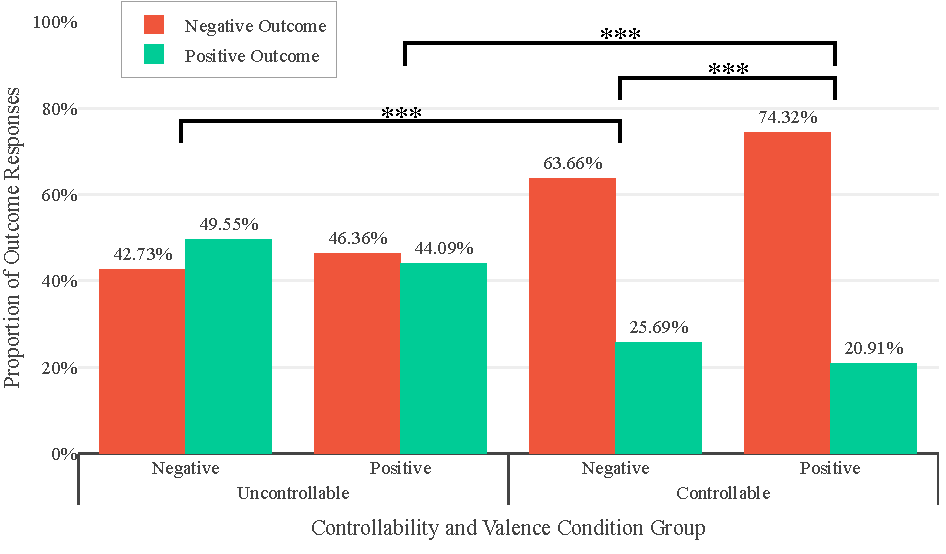
\includegraphics[width=0.9\textwidth]{../_kallysto/figs/4_Experiment1_Analysis.ipynb/ValenceMain.pdf}
        \caption{Valence of unexpected  events, reported as negative and positive outcomes, in the four conditions of the study. *** p $\leq$ 0.001}
        \label{ValenceMain}
    \end{figure}
}


% Uid: 1650461186.934664
% Created: 14:26:26 04/20/22 IST
% Exported: 14:26:26 04/20/22 IST
% Title: control_report
% Notebook: ../../../4_Experiment1_Analysis.ipynb
% Image file: ../_kallysto/figs/4_Experiment1_Analysis.ipynb/NegLogOddsValenceMaterialsChart.pdf
% Data file: ../_kallysto/data/4_Experiment1_Analysis.ipynb/NegLogOddsValenceMaterialsChart.fig.csv
\providecommand{\NegLogOddsValenceMaterialsChart}{
dummy}
\renewcommand{\NegLogOddsValenceMaterialsChart}{
    \begin{figure}
        \center
        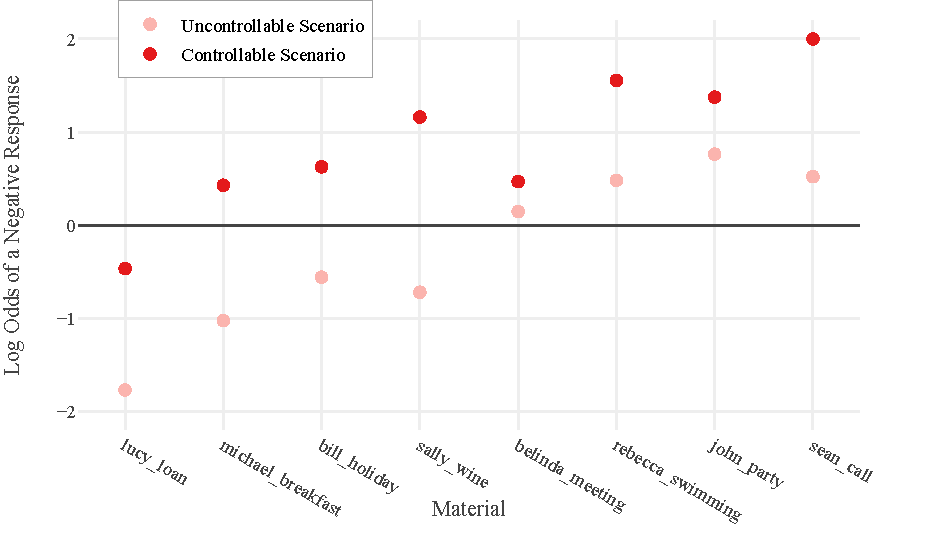
\includegraphics[width=1\textwidth]{../_kallysto/figs/4_Experiment1_Analysis.ipynb/NegLogOddsValenceMaterialsChart.pdf}
        \caption{Log odds of reporting a negative outcome (i.e., the negativity index) for the uncontrollable and controllable versions of each material-scenario in the study.}
        \label{NegLogOddsValenceMaterialsChart}
    \end{figure}
}


% Uid: 1650461187.4421709
% Created: 14:26:27 04/20/22 IST
% Exported: 14:26:27 04/20/22 IST
% Title: control_report
% Notebook: ../../../4_Experiment1_Analysis.ipynb
% Data file: ../_kallysto/data/4_Experiment1_Analysis.ipynb/uncontrollableoverallprop.txt
\providecommand{\uncontrollableoverallprop}{
dummy}
\renewcommand{\uncontrollableoverallprop}{
55.02}


% Uid: 1650461187.443721
% Created: 14:26:27 04/20/22 IST
% Exported: 14:26:27 04/20/22 IST
% Title: control_report
% Notebook: ../../../4_Experiment1_Analysis.ipynb
% Data file: ../_kallysto/data/4_Experiment1_Analysis.ipynb/controllableoverallprop.txt
\providecommand{\controllableoverallprop}{
dummy}
\renewcommand{\controllableoverallprop}{
25.46}


% Uid: 1650461187.44505
% Created: 14:26:27 04/20/22 IST
% Exported: 14:26:27 04/20/22 IST
% Title: control_report
% Notebook: ../../../4_Experiment1_Analysis.ipynb
% Data file: ../_kallysto/data/4_Experiment1_Analysis.ipynb/neithercontroloverallprop.txt
\providecommand{\neithercontroloverallprop}{
dummy}
\renewcommand{\neithercontroloverallprop}{
19.52}


% Uid: 1650461187.6197839
% Created: 14:26:27 04/20/22 IST
% Exported: 14:26:27 04/20/22 IST
% Title: control_report
% Notebook: ../../../4_Experiment1_Analysis.ipynb
% Data file: ../_kallysto/data/4_Experiment1_Analysis.ipynb/controllablechi.txt
\providecommand{\controllablechi}{
dummy}
\renewcommand{\controllablechi}{
\chi^2(6, N=1752)=19.49, p = 0.003, v=0.075}


% Uid: 1650461187.625877
% Created: 14:26:27 04/20/22 IST
% Exported: 14:26:27 04/20/22 IST
% Title: control_report
% Notebook: ../../../4_Experiment1_Analysis.ipynb
% Data file: ../_kallysto/data/4_Experiment1_Analysis.ipynb/controllablebyvalencecondchi.txt
\providecommand{\controllablebyvalencecondchi}{
dummy}
\renewcommand{\controllablebyvalencecondchi}{
\chi^2(2, N=1752)=18.13, p < .001, v=0.102}


% Uid: 1650461187.6557481
% Created: 14:26:27 04/20/22 IST
% Exported: 14:26:27 04/20/22 IST
% Title: control_report
% Notebook: ../../../4_Experiment1_Analysis.ipynb
% Data file: ../_kallysto/data/4_Experiment1_Analysis.ipynb/controllablebymeanscondchi.txt
\providecommand{\controllablebymeanscondchi}{
dummy}
\renewcommand{\controllablebymeanscondchi}{
\chi^2(2, N=1752)=0.59, p = 0.743, v=0.018}


% Uid: 1650461187.665906
% Created: 14:26:27 04/20/22 IST
% Exported: 14:26:27 04/20/22 IST
% Title: control_report
% Notebook: ../../../4_Experiment1_Analysis.ipynb
% Data file: ../_kallysto/data/4_Experiment1_Analysis.ipynb/negativeabsentnegativepresentcontrollablechi.txt
\providecommand{\negativeabsentnegativepresentcontrollablechi}{
dummy}
\renewcommand{\negativeabsentnegativepresentcontrollablechi}{
\chi^2(2, N=872)=1.20, p = 0.548, v=0.037}


% Uid: 1650461187.6750028
% Created: 14:26:27 04/20/22 IST
% Exported: 14:26:27 04/20/22 IST
% Title: control_report
% Notebook: ../../../4_Experiment1_Analysis.ipynb
% Data file: ../_kallysto/data/4_Experiment1_Analysis.ipynb/negativeabsentpositiveabsentcontrollablechi.txt
\providecommand{\negativeabsentpositiveabsentcontrollablechi}{
dummy}
\renewcommand{\negativeabsentpositiveabsentcontrollablechi}{
\chi^2(2, N=880)=11.79, p < .001, v=0.116}


% Uid: 1650461187.682306
% Created: 14:26:27 04/20/22 IST
% Exported: 14:26:27 04/20/22 IST
% Title: control_report
% Notebook: ../../../4_Experiment1_Analysis.ipynb
% Data file: ../_kallysto/data/4_Experiment1_Analysis.ipynb/negativeabsentpositivepresentcontrollablechi.txt
\providecommand{\negativeabsentpositivepresentcontrollablechi}{
dummy}
\renewcommand{\negativeabsentpositivepresentcontrollablechi}{
\chi^2(2, N=880)=10.44, p < .001, v=0.109}


% Uid: 1650461187.6915252
% Created: 14:26:27 04/20/22 IST
% Exported: 14:26:27 04/20/22 IST
% Title: control_report
% Notebook: ../../../4_Experiment1_Analysis.ipynb
% Data file: ../_kallysto/data/4_Experiment1_Analysis.ipynb/negativepresentpositiveabsentcontrollablechi.txt
\providecommand{\negativepresentpositiveabsentcontrollablechi}{
dummy}
\renewcommand{\negativepresentpositiveabsentcontrollablechi}{
\chi^2(2, N=872)=8.09, p < .001, v=0.096}


% Uid: 1650461187.7081459
% Created: 14:26:27 04/20/22 IST
% Exported: 14:26:27 04/20/22 IST
% Title: control_report
% Notebook: ../../../4_Experiment1_Analysis.ipynb
% Data file: ../_kallysto/data/4_Experiment1_Analysis.ipynb/negativepresentpositivepresentcontrollablechi.txt
\providecommand{\negativepresentpositivepresentcontrollablechi}{
dummy}
\renewcommand{\negativepresentpositivepresentcontrollablechi}{
\chi^2(2, N=872)=6.96, p < .001, v=0.089}


% Uid: 1650461187.7174022
% Created: 14:26:27 04/20/22 IST
% Exported: 14:26:27 04/20/22 IST
% Title: control_report
% Notebook: ../../../4_Experiment1_Analysis.ipynb
% Data file: ../_kallysto/data/4_Experiment1_Analysis.ipynb/positiveabsentpositivepresentcontrollablechi.txt
\providecommand{\positiveabsentpositivepresentcontrollablechi}{
dummy}
\renewcommand{\positiveabsentpositivepresentcontrollablechi}{
\chi^2(2, N=880)=0.04, p = 0.978, v=0.007}


% Uid: 1650461187.727592
% Created: 14:26:27 04/20/22 IST
% Exported: 14:26:27 04/20/22 IST
% Title: control_report
% Notebook: ../../../4_Experiment1_Analysis.ipynb
% Data file: ../_kallysto/data/4_Experiment1_Analysis.ipynb/johnpartycontrollablechi.txt
\providecommand{\johnpartycontrollablechi}{
dummy}
\renewcommand{\johnpartycontrollablechi}{
\chi^2(6, N=219)=11.99, p = 0.062, v=0.165}


% Uid: 1650461187.731976
% Created: 14:26:27 04/20/22 IST
% Exported: 14:26:27 04/20/22 IST
% Title: control_report
% Notebook: ../../../4_Experiment1_Analysis.ipynb
% Data file: ../_kallysto/data/4_Experiment1_Analysis.ipynb/billholidaycontrollablechi.txt
\providecommand{\billholidaycontrollablechi}{
dummy}
\renewcommand{\billholidaycontrollablechi}{
\chi^2(6, N=219)=3.72, p = 0.715, v=0.092}


% Uid: 1650461187.736166
% Created: 14:26:27 04/20/22 IST
% Exported: 14:26:27 04/20/22 IST
% Title: control_report
% Notebook: ../../../4_Experiment1_Analysis.ipynb
% Data file: ../_kallysto/data/4_Experiment1_Analysis.ipynb/rebeccaswimmingcontrollablechi.txt
\providecommand{\rebeccaswimmingcontrollablechi}{
dummy}
\renewcommand{\rebeccaswimmingcontrollablechi}{
\chi^2(6, N=219)=21.27, p < .001, v=0.220}


% Uid: 1650461187.741392
% Created: 14:26:27 04/20/22 IST
% Exported: 14:26:27 04/20/22 IST
% Title: control_report
% Notebook: ../../../4_Experiment1_Analysis.ipynb
% Data file: ../_kallysto/data/4_Experiment1_Analysis.ipynb/sallywinecontrollablechi.txt
\providecommand{\sallywinecontrollablechi}{
dummy}
\renewcommand{\sallywinecontrollablechi}{
\chi^2(6, N=219)=24.68, p < .001, v=0.237}


% Uid: 1650461187.745301
% Created: 14:26:27 04/20/22 IST
% Exported: 14:26:27 04/20/22 IST
% Title: control_report
% Notebook: ../../../4_Experiment1_Analysis.ipynb
% Data file: ../_kallysto/data/4_Experiment1_Analysis.ipynb/belindameetingcontrollablechi.txt
\providecommand{\belindameetingcontrollablechi}{
dummy}
\renewcommand{\belindameetingcontrollablechi}{
\chi^2(6, N=219)=3.39, p = 0.758, v=0.088}


% Uid: 1650461187.748849
% Created: 14:26:27 04/20/22 IST
% Exported: 14:26:27 04/20/22 IST
% Title: control_report
% Notebook: ../../../4_Experiment1_Analysis.ipynb
% Data file: ../_kallysto/data/4_Experiment1_Analysis.ipynb/michaelbreakfastcontrollablechi.txt
\providecommand{\michaelbreakfastcontrollablechi}{
dummy}
\renewcommand{\michaelbreakfastcontrollablechi}{
\chi^2(6, N=219)=14.64, p < .001, v=0.183}


% Uid: 1650461187.754519
% Created: 14:26:27 04/20/22 IST
% Exported: 14:26:27 04/20/22 IST
% Title: control_report
% Notebook: ../../../4_Experiment1_Analysis.ipynb
% Data file: ../_kallysto/data/4_Experiment1_Analysis.ipynb/lucyloancontrollablechi.txt
\providecommand{\lucyloancontrollablechi}{
dummy}
\renewcommand{\lucyloancontrollablechi}{
\chi^2(6, N=219)=11.10, p = 0.085, v=0.159}


% Uid: 1650461187.760433
% Created: 14:26:27 04/20/22 IST
% Exported: 14:26:27 04/20/22 IST
% Title: control_report
% Notebook: ../../../4_Experiment1_Analysis.ipynb
% Data file: ../_kallysto/data/4_Experiment1_Analysis.ipynb/seancallcontrollablechi.txt
\providecommand{\seancallcontrollablechi}{
dummy}
\renewcommand{\seancallcontrollablechi}{
\chi^2(6, N=219)=3.21, p = 0.782, v=0.086}


% Uid: 1650461187.7713878
% Created: 14:26:27 04/20/22 IST
% Exported: 14:26:27 04/20/22 IST
% Title: control_report
% Notebook: ../../../4_Experiment1_Analysis.ipynb
% Data file: ../_kallysto/data/4_Experiment1_Analysis.ipynb/johnpartycontrollablevalenceconditionchi.txt
\providecommand{\johnpartycontrollablevalenceconditionchi}{
dummy}
\renewcommand{\johnpartycontrollablevalenceconditionchi}{
\chi^2(2, N=219)=9.49, p < .001, v=0.208}


% Uid: 1650461187.77488
% Created: 14:26:27 04/20/22 IST
% Exported: 14:26:27 04/20/22 IST
% Title: control_report
% Notebook: ../../../4_Experiment1_Analysis.ipynb
% Data file: ../_kallysto/data/4_Experiment1_Analysis.ipynb/billholidaycontrollablevalenceconditionchi.txt
\providecommand{\billholidaycontrollablevalenceconditionchi}{
dummy}
\renewcommand{\billholidaycontrollablevalenceconditionchi}{
\chi^2(2, N=219)=0.31, p = 0.855, v=0.038}


% Uid: 1650461187.7782469
% Created: 14:26:27 04/20/22 IST
% Exported: 14:26:27 04/20/22 IST
% Title: control_report
% Notebook: ../../../4_Experiment1_Analysis.ipynb
% Data file: ../_kallysto/data/4_Experiment1_Analysis.ipynb/rebeccaswimmingcontrollablevalenceconditionchi.txt
\providecommand{\rebeccaswimmingcontrollablevalenceconditionchi}{
dummy}
\renewcommand{\rebeccaswimmingcontrollablevalenceconditionchi}{
\chi^2(2, N=219)=9.02, p < .001, v=0.203}


% Uid: 1650461187.781674
% Created: 14:26:27 04/20/22 IST
% Exported: 14:26:27 04/20/22 IST
% Title: control_report
% Notebook: ../../../4_Experiment1_Analysis.ipynb
% Data file: ../_kallysto/data/4_Experiment1_Analysis.ipynb/sallywinecontrollablevalenceconditionchi.txt
\providecommand{\sallywinecontrollablevalenceconditionchi}{
dummy}
\renewcommand{\sallywinecontrollablevalenceconditionchi}{
\chi^2(2, N=219)=12.43, p < .001, v=0.238}


% Uid: 1650461187.785277
% Created: 14:26:27 04/20/22 IST
% Exported: 14:26:27 04/20/22 IST
% Title: control_report
% Notebook: ../../../4_Experiment1_Analysis.ipynb
% Data file: ../_kallysto/data/4_Experiment1_Analysis.ipynb/belindameetingcontrollablevalenceconditionchi.txt
\providecommand{\belindameetingcontrollablevalenceconditionchi}{
dummy}
\renewcommand{\belindameetingcontrollablevalenceconditionchi}{
\chi^2(2, N=219)=0.35, p = 0.838, v=0.040}


% Uid: 1650461187.7914822
% Created: 14:26:27 04/20/22 IST
% Exported: 14:26:27 04/20/22 IST
% Title: control_report
% Notebook: ../../../4_Experiment1_Analysis.ipynb
% Data file: ../_kallysto/data/4_Experiment1_Analysis.ipynb/michaelbreakfastcontrollablevalenceconditionchi.txt
\providecommand{\michaelbreakfastcontrollablevalenceconditionchi}{
dummy}
\renewcommand{\michaelbreakfastcontrollablevalenceconditionchi}{
\chi^2(2, N=219)=1.64, p = 0.441, v=0.086}


% Uid: 1650461187.7984152
% Created: 14:26:27 04/20/22 IST
% Exported: 14:26:27 04/20/22 IST
% Title: control_report
% Notebook: ../../../4_Experiment1_Analysis.ipynb
% Data file: ../_kallysto/data/4_Experiment1_Analysis.ipynb/lucyloancontrollablevalenceconditionchi.txt
\providecommand{\lucyloancontrollablevalenceconditionchi}{
dummy}
\renewcommand{\lucyloancontrollablevalenceconditionchi}{
\chi^2(2, N=219)=10.66, p < .001, v=0.221}


% Uid: 1650461187.806568
% Created: 14:26:27 04/20/22 IST
% Exported: 14:26:27 04/20/22 IST
% Title: control_report
% Notebook: ../../../4_Experiment1_Analysis.ipynb
% Data file: ../_kallysto/data/4_Experiment1_Analysis.ipynb/seancallcontrollablevalenceconditionchi.txt
\providecommand{\seancallcontrollablevalenceconditionchi}{
dummy}
\renewcommand{\seancallcontrollablevalenceconditionchi}{
\chi^2(2, N=219)=2.18, p = 0.336, v=0.100}


% Uid: 1650461187.829783
% Created: 14:26:27 04/20/22 IST
% Exported: 14:26:27 04/20/22 IST
% Title: control_report
% Notebook: ../../../4_Experiment1_Analysis.ipynb
% Data file: ../_kallysto/data/4_Experiment1_Analysis.ipynb/johnpartycontrollablemeansconditionchi.txt
\providecommand{\johnpartycontrollablemeansconditionchi}{
dummy}
\renewcommand{\johnpartycontrollablemeansconditionchi}{
\chi^2(2, N=219)=0.88, p = 0.645, v=0.063}


% Uid: 1650461187.8382452
% Created: 14:26:27 04/20/22 IST
% Exported: 14:26:27 04/20/22 IST
% Title: control_report
% Notebook: ../../../4_Experiment1_Analysis.ipynb
% Data file: ../_kallysto/data/4_Experiment1_Analysis.ipynb/billholidaycontrollablemeansconditionchi.txt
\providecommand{\billholidaycontrollablemeansconditionchi}{
dummy}
\renewcommand{\billholidaycontrollablemeansconditionchi}{
\chi^2(2, N=219)=2.55, p = 0.280, v=0.108}


% Uid: 1650461187.846596
% Created: 14:26:27 04/20/22 IST
% Exported: 14:26:27 04/20/22 IST
% Title: control_report
% Notebook: ../../../4_Experiment1_Analysis.ipynb
% Data file: ../_kallysto/data/4_Experiment1_Analysis.ipynb/rebeccaswimmingcontrollablemeansconditionchi.txt
\providecommand{\rebeccaswimmingcontrollablemeansconditionchi}{
dummy}
\renewcommand{\rebeccaswimmingcontrollablemeansconditionchi}{
\chi^2(2, N=219)=11.73, p < .001, v=0.231}


% Uid: 1650461187.854589
% Created: 14:26:27 04/20/22 IST
% Exported: 14:26:27 04/20/22 IST
% Title: control_report
% Notebook: ../../../4_Experiment1_Analysis.ipynb
% Data file: ../_kallysto/data/4_Experiment1_Analysis.ipynb/sallywinecontrollablemeansconditionchi.txt
\providecommand{\sallywinecontrollablemeansconditionchi}{
dummy}
\renewcommand{\sallywinecontrollablemeansconditionchi}{
\chi^2(2, N=219)=10.00, p < .001, v=0.214}


% Uid: 1650461187.8619132
% Created: 14:26:27 04/20/22 IST
% Exported: 14:26:27 04/20/22 IST
% Title: control_report
% Notebook: ../../../4_Experiment1_Analysis.ipynb
% Data file: ../_kallysto/data/4_Experiment1_Analysis.ipynb/belindameetingcontrollablemeansconditionchi.txt
\providecommand{\belindameetingcontrollablemeansconditionchi}{
dummy}
\renewcommand{\belindameetingcontrollablemeansconditionchi}{
\chi^2(2, N=219)=0.97, p = 0.615, v=0.067}


% Uid: 1650461187.867481
% Created: 14:26:27 04/20/22 IST
% Exported: 14:26:27 04/20/22 IST
% Title: control_report
% Notebook: ../../../4_Experiment1_Analysis.ipynb
% Data file: ../_kallysto/data/4_Experiment1_Analysis.ipynb/michaelbreakfastcontrollablemeansconditionchi.txt
\providecommand{\michaelbreakfastcontrollablemeansconditionchi}{
dummy}
\renewcommand{\michaelbreakfastcontrollablemeansconditionchi}{
\chi^2(2, N=219)=3.72, p = 0.156, v=0.130}


% Uid: 1650461187.8717551
% Created: 14:26:27 04/20/22 IST
% Exported: 14:26:27 04/20/22 IST
% Title: control_report
% Notebook: ../../../4_Experiment1_Analysis.ipynb
% Data file: ../_kallysto/data/4_Experiment1_Analysis.ipynb/lucyloancontrollablemeansconditionchi.txt
\providecommand{\lucyloancontrollablemeansconditionchi}{
dummy}
\renewcommand{\lucyloancontrollablemeansconditionchi}{
\chi^2(2, N=219)=0.40, p = 0.817, v=0.043}


% Uid: 1650461187.8796391
% Created: 14:26:27 04/20/22 IST
% Exported: 14:26:27 04/20/22 IST
% Title: control_report
% Notebook: ../../../4_Experiment1_Analysis.ipynb
% Data file: ../_kallysto/data/4_Experiment1_Analysis.ipynb/seancallcontrollablemeansconditionchi.txt
\providecommand{\seancallcontrollablemeansconditionchi}{
dummy}
\renewcommand{\seancallcontrollablemeansconditionchi}{
\chi^2(2, N=219)=0.98, p = 0.611, v=0.067}


% Uid: 1650461187.952245
% Created: 14:26:27 04/20/22 IST
% Exported: 14:26:27 04/20/22 IST
% Title: control_report
% Notebook: ../../../4_Experiment1_Analysis.ipynb
% Image file: ../_kallysto/figs/4_Experiment1_Analysis.ipynb/ControlMain.pdf
% Data file: ../_kallysto/data/4_Experiment1_Analysis.ipynb/ControlMain.fig.csv
\providecommand{\ControlMain}{
dummy}
\renewcommand{\ControlMain}{
    \begin{figure}
        \center
        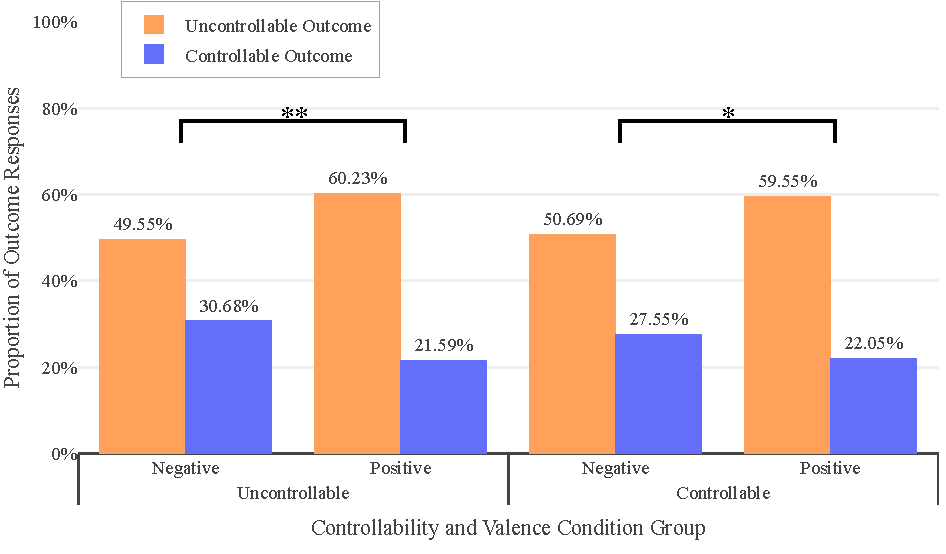
\includegraphics[width=1\textwidth]{../_kallysto/figs/4_Experiment1_Analysis.ipynb/ControlMain.pdf}
        \caption{Controllability of unexpected  events, reported as uncontrollable and controllable outcomes, in the four conditions of the study. * p<.05, ** p<.005}
        \label{ControlMain}
    \end{figure}
}


% Uid: 1650461188.459742
% Created: 14:26:28 04/20/22 IST
% Exported: 14:26:28 04/20/22 IST
% Title: control_report
% Notebook: ../../../4_Experiment1_Analysis.ipynb
% Data file: ../_kallysto/data/4_Experiment1_Analysis.ipynb/negativelogoddsuncontrollable.txt
\providecommand{\negativelogoddsuncontrollable}{
dummy}
\renewcommand{\negativelogoddsuncontrollable}{
0.005}


% Uid: 1650461188.461941
% Created: 14:26:28 04/20/22 IST
% Exported: 14:26:28 04/20/22 IST
% Title: control_report
% Notebook: ../../../4_Experiment1_Analysis.ipynb
% Data file: ../_kallysto/data/4_Experiment1_Analysis.ipynb/positivelogoddsuncontrollable.txt
\providecommand{\positivelogoddsuncontrollable}{
dummy}
\renewcommand{\positivelogoddsuncontrollable}{
0.401}


% Uid: 1650461188.682935
% Created: 14:26:28 04/20/22 IST
% Exported: 14:26:28 04/20/22 IST
% Title: control_report
% Notebook: ../../../4_Experiment1_Analysis.ipynb
% Image file: ../_kallysto/figs/4_Experiment1_Analysis.ipynb/UncontrollableLogOddsValenceMaterialsChart.pdf
% Data file: ../_kallysto/data/4_Experiment1_Analysis.ipynb/UncontrollableLogOddsValenceMaterialsChart.fig.csv
\providecommand{\UncontrollableLogOddsValenceMaterialsChart}{
dummy}
\renewcommand{\UncontrollableLogOddsValenceMaterialsChart}{
    \begin{figure}
        \center
        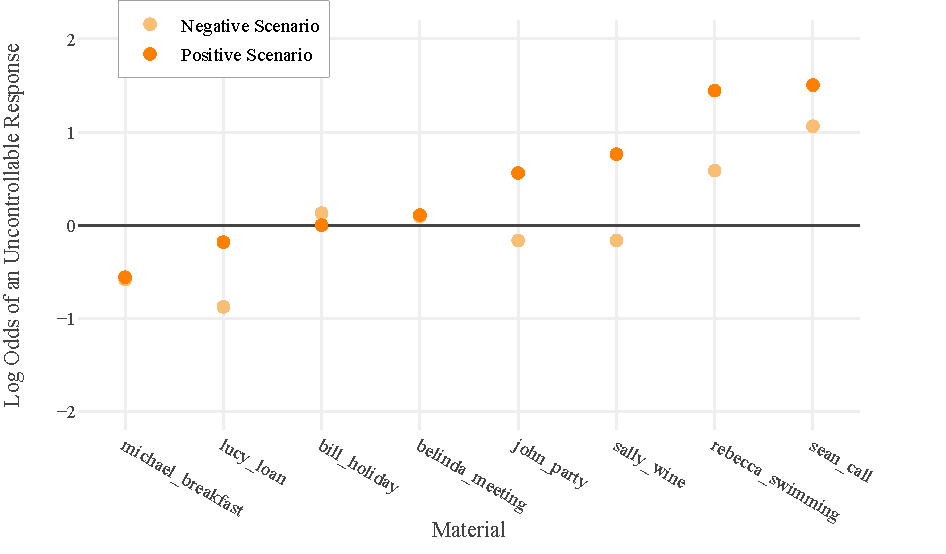
\includegraphics[width=1\textwidth]{../_kallysto/figs/4_Experiment1_Analysis.ipynb/UncontrollableLogOddsValenceMaterialsChart.pdf}
        \caption{Log odds of reporting an uncontrollable outcome (i.e., the uncontrollability index) for the negative- and positive-valenced versions of each material-scenario in the study.}
        \label{UncontrollableLogOddsValenceMaterialsChart}
    \end{figure}
}


% Uid: 1650461189.577734
% Created: 14:26:29 04/20/22 IST
% Exported: 14:26:29 04/20/22 IST
% Title: control_report
% Notebook: ../../../4_Experiment1_Analysis.ipynb
% Image file: ../_kallysto/figs/4_Experiment1_Analysis.ipynb/interxoverallbar.pdf
% Data file: ../_kallysto/data/4_Experiment1_Analysis.ipynb/interxoverallbar.fig.csv
\providecommand{\interxoverallbar}{
dummy}
\renewcommand{\interxoverallbar}{
    \begin{figure}
        \center
        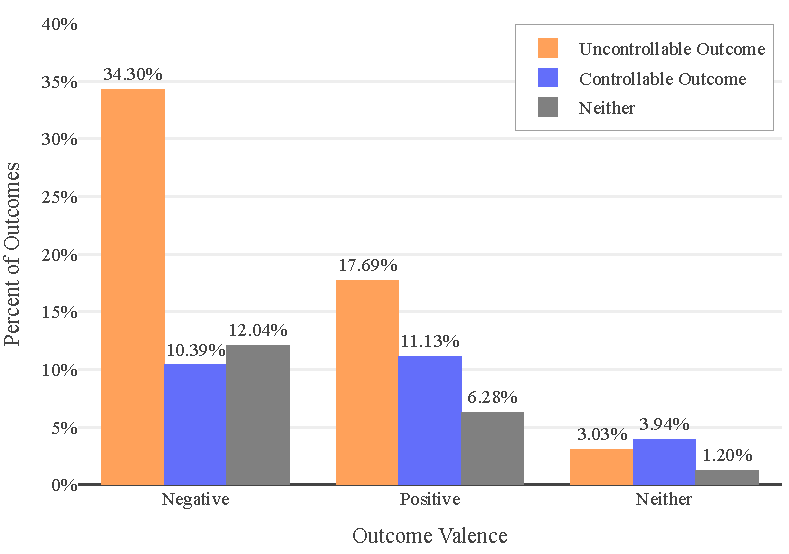
\includegraphics[width=1\textwidth]{../_kallysto/figs/4_Experiment1_Analysis.ipynb/interxoverallbar.pdf}
        \caption{Percent of each outcome controllability by outcome valence.}
        \label{interxoverallbar}
    \end{figure}
}


% Uid: 1650461190.640324
% Created: 14:26:30 04/20/22 IST
% Exported: 14:26:30 04/20/22 IST
% Title: control_report
% Notebook: ../../../4_Experiment1_Analysis.ipynb
% Image file: ../_kallysto/figs/4_Experiment1_Analysis.ipynb/interxHbar.pdf
% Data file: ../_kallysto/data/4_Experiment1_Analysis.ipynb/interxHbar.fig.csv
\providecommand{\interxHbar}{
dummy}
\renewcommand{\interxHbar}{
    \begin{figure}
        \center
        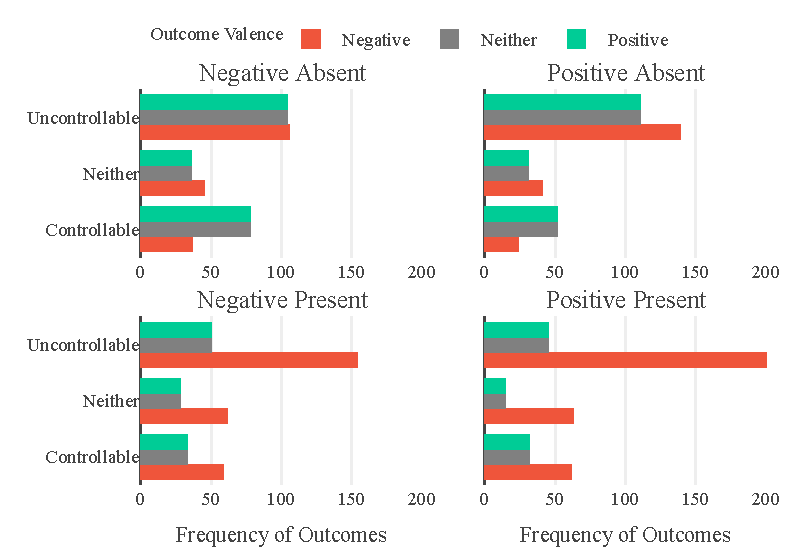
\includegraphics[width=1\textwidth]{../_kallysto/figs/4_Experiment1_Analysis.ipynb/interxHbar.pdf}
        \caption{Categories of unexpected events, reported by outcome-valence (positive, negative, neither) and outcome-controllability (uncontrollable, controllable, neither), collapsing across the four conditions in the study.}
        \label{interxHbar}
    \end{figure}
}


% Uid: 1650461191.47028
% Created: 14:26:31 04/20/22 IST
% Exported: 14:26:31 04/20/22 IST
% Title: control_report
% Notebook: ../../../4_Experiment1_Analysis.ipynb
% Data file: ../_kallysto/data/4_Experiment1_Analysis.ipynb/NegativeAbsentValenceOutcomeByControlOutcomeChi.txt
\providecommand{\NegativeAbsentValenceOutcomeByControlOutcomeChi}{
dummy}
\renewcommand{\NegativeAbsentValenceOutcomeByControlOutcomeChi}{
\chi^2(4, N=440)=27.11, p < .001, v=0.176}


% Uid: 1650461191.523146
% Created: 14:26:31 04/20/22 IST
% Exported: 14:26:31 04/20/22 IST
% Title: control_report
% Notebook: ../../../4_Experiment1_Analysis.ipynb
% Data file: ../_kallysto/data/4_Experiment1_Analysis.ipynb/NegativePresentValenceOutcomeByControlOutcomeChi.txt
\providecommand{\NegativePresentValenceOutcomeByControlOutcomeChi}{
dummy}
\renewcommand{\NegativePresentValenceOutcomeByControlOutcomeChi}{
\chi^2(4, N=432)=29.23, p < .001, v=0.184}


% Uid: 1650461191.573882
% Created: 14:26:31 04/20/22 IST
% Exported: 14:26:31 04/20/22 IST
% Title: control_report
% Notebook: ../../../4_Experiment1_Analysis.ipynb
% Data file: ../_kallysto/data/4_Experiment1_Analysis.ipynb/PositiveAbsentValenceOutcomeByControlOutcomeChi.txt
\providecommand{\PositiveAbsentValenceOutcomeByControlOutcomeChi}{
dummy}
\renewcommand{\PositiveAbsentValenceOutcomeByControlOutcomeChi}{
\chi^2(4, N=440)=29.57, p < .001, v=0.183}


% Uid: 1650461191.624331
% Created: 14:26:31 04/20/22 IST
% Exported: 14:26:31 04/20/22 IST
% Title: control_report
% Notebook: ../../../4_Experiment1_Analysis.ipynb
% Data file: ../_kallysto/data/4_Experiment1_Analysis.ipynb/PositivePresentValenceOutcomeByControlOutcomeChi.txt
\providecommand{\PositivePresentValenceOutcomeByControlOutcomeChi}{
dummy}
\renewcommand{\PositivePresentValenceOutcomeByControlOutcomeChi}{
\chi^2(4, N=440)=11.52, p = 0.021, v=0.114}


% Uid: 1650461191.9091609
% Created: 14:26:31 04/20/22 IST
% Exported: 14:26:31 04/20/22 IST
% Title: control_report
% Notebook: ../../../4_Experiment1_Analysis.ipynb
% Image file: ../_kallysto/figs/4_Experiment1_Analysis.ipynb/RatingsByConditionHeatmap.pdf
% Data file: ../_kallysto/data/4_Experiment1_Analysis.ipynb/RatingsByConditionHeatmap.fig.csv
\providecommand{\RatingsByConditionHeatmap}{
dummy}
\renewcommand{\RatingsByConditionHeatmap}{
    \begin{figure}
        \center
        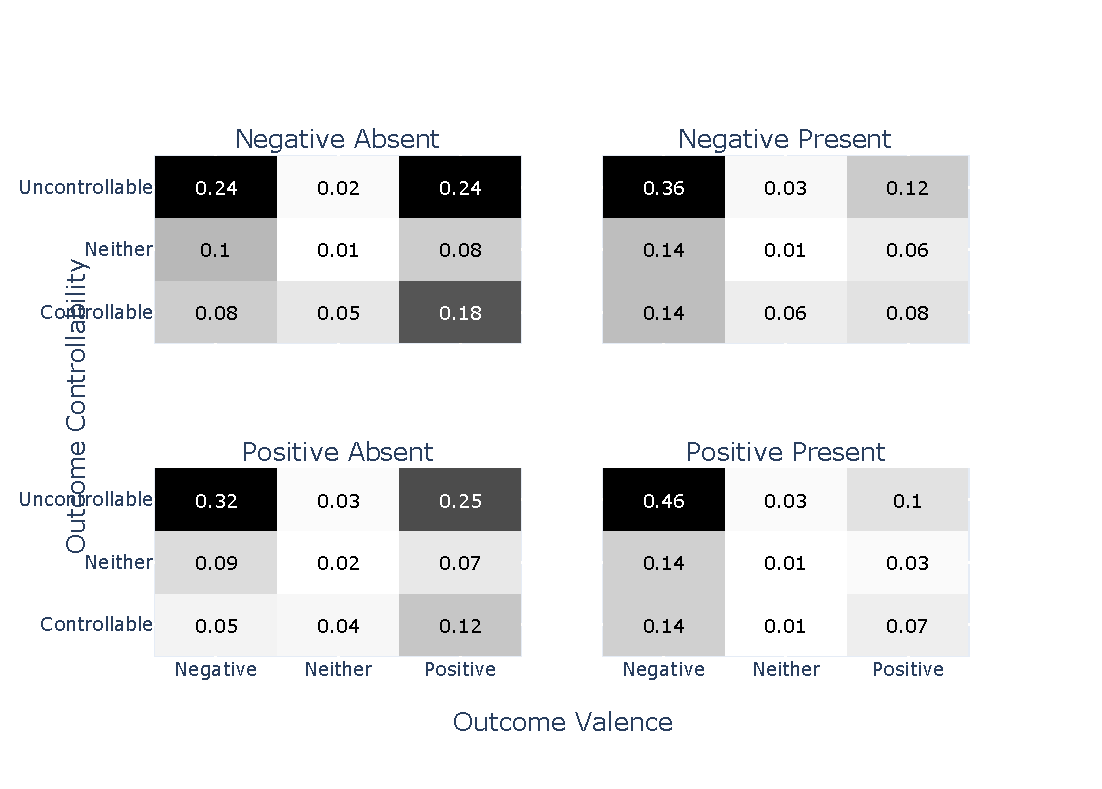
\includegraphics[width=1\textwidth]{../_kallysto/figs/4_Experiment1_Analysis.ipynb/RatingsByConditionHeatmap.pdf}
        \caption{Crosstabs of outcome controllability and valence ratings by condition.}
        \label{RatingsByConditionHeatmap}
    \end{figure}
}


% Uid: 1650461192.667115
% Created: 14:26:32 04/20/22 IST
% Exported: 14:26:32 04/20/22 IST
% Title: control_report
% Notebook: ../../../4_Experiment1_Analysis.ipynb
% Image file: ../_kallysto/figs/4_Experiment1_Analysis.ipynb/InteractionSubplots.pdf
% Data file: ../_kallysto/data/4_Experiment1_Analysis.ipynb/InteractionSubplots.fig.csv
\providecommand{\InteractionSubplots}{
dummy}
\renewcommand{\InteractionSubplots}{
    \begin{figure}
        \center
        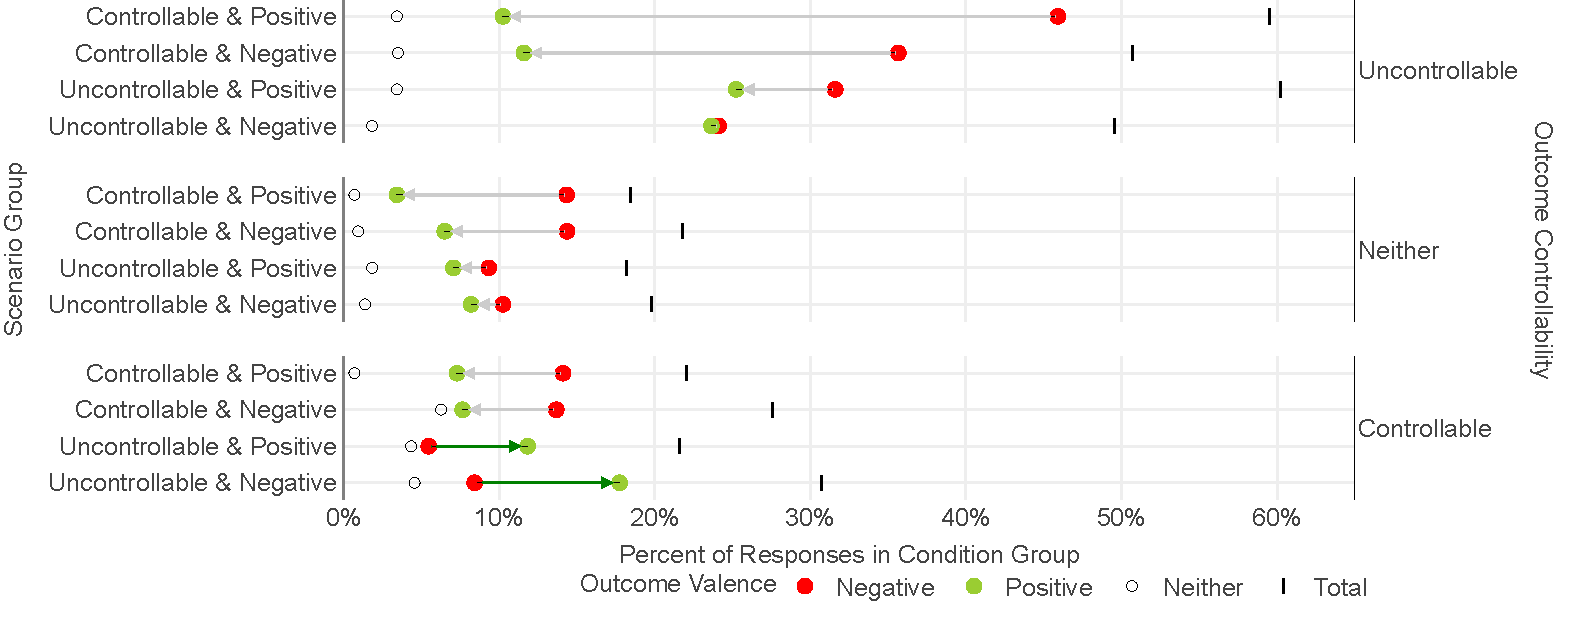
\includegraphics[width=1\textwidth]{../_kallysto/figs/4_Experiment1_Analysis.ipynb/InteractionSubplots.pdf}
        \caption{Responses as percentage of total responses in a given Experimental Group labeled as positive, negative, and neither split by outcome controllability, and for each experimental group. Respective total percentage of responses labeled as each outcome controllability label shown as a single vertical black line. Arrows show the direction from negative to positive percentages. The arrows showing an increase in percentage of positive outcomes relative to negative outcomes are highlighted for the controllable outcomes in the Means Absent experimental groups.}
        \label{InteractionSubplots}
    \end{figure}
}


